\section{Deep learning}
\subsection{Perceptron. Multi-layer Perceptron. The fixed-size computing paradigm.}
There are already too many technical texts about the mathematical behind Perceptron and Multi-layer Perceptron. In this section, we will take a pictorial look at it, starting from matrix multiplication.

\paragraph{Perceptron} is defined as a function that maps its input $\vect{x}$
(a real-valued vector) to an output value $y$(a single binary value):
\begin{align}
  y = \vect{W} \times \vect{x} + \text{bias}
\end{align}

\begin{figure*}[t]
  \centering
  \begin{subfigure}[t]{0.45\textwidth}
    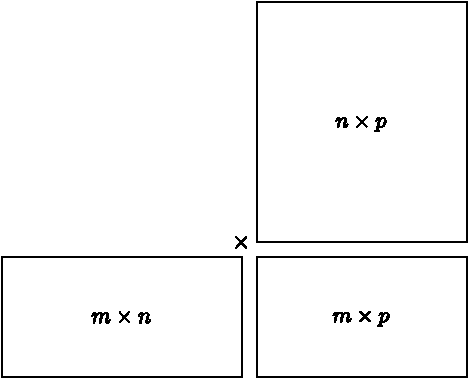
\includegraphics[width=0.99\textwidth]{figures/matmul.pdf}
    \caption{Matrix multiplication.}
    \label{fig:matmul}
	\end{subfigure}
	\begin{subfigure}[t]{0.45\textwidth}
    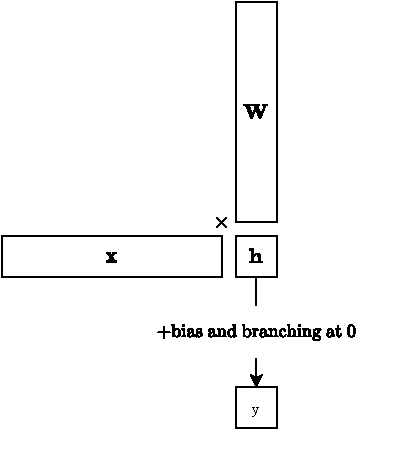
\includegraphics[width=0.99\textwidth]{figures/perceptron.pdf}
    \caption{A perceptron}
    \label{fig:perceptron}
	\end{subfigure}
	\begin{subfigure}[b]{0.9\textwidth}
    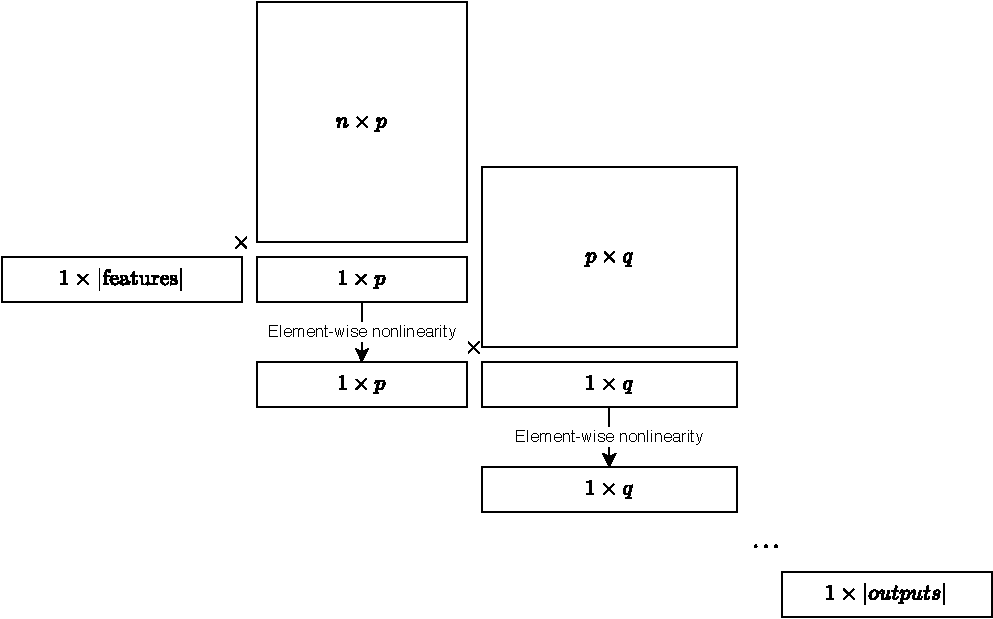
\includegraphics[width=0.99\textwidth]{figures/deep_matmul.pdf}
    \caption{Multi-layer Perceptron, viewed as a series of matrix transformation.}
    \label{fig:deep_matmul}
	\end{subfigure}


  \caption{Visualization of matrix multiplication, perceptron, and multi-layer perceptron.}
  % \label{fig:vis_ind_gen}
\end{figure*}
\subsection{Recurrent-neural network. Tree LSTM}
In many tasks, we need to process inputs of arbitrary length, to predict outputs also of arbitrary length (often called \emph{sequence-to-sequence} problems). There are multiple ways to make sequential inputs to work in the fixed-size paradigm, such as \emph{padding} (add dummy values to the inputs to make sure they are all of the same length), \emph{same length batching} (sort inputs by size and process inputs of the same size together), among others. However, those approaches doesn't help with handling sequential outputs. A better approach is \emph{recurrent neural networks} (RNNs). An RNN defines a function
\begin{align}
\vect{h}^t = f(\vect{h}^{t-1}, \vect{x}^{t})
\end{align}
in which $f$ is our matrix transformation. 
%% Recurrent neural networks (RNNs) are widely used in natural language processingtasks, especially speech recognition and machine translation. The primary goal ofRNNs is to approximate the mapping from a sequence of inputsx(1),...,x(t)to eithera single outputyor a sequence of outputsy(1),...,y(t). An RNN defines a mappingh(t)=f(h(t−1),x(t);θ)(2.2)whereh(t)is the hidden state, from which the final outputy(t)can be computed byeither a non-linear transformation or an MLP.11
%% Popular RNN models.A simple RNN model can bef(h(t−1),x(t);θ) =tanh(Wx(t)+Uh(t−1)+b)(2.3)whereθ=  [W,U,b]. The key issue of such a simple form is that the long-termdependencies are hard to capture, which makes training extremely difficult. Toaddress this issue, a commonly used RNN model is the long short-term memorynetwork (LSTM) [89], which introduces amemory cell with various gatesto preservestate over a long sequence.LSTM maintains two states — the original hidden state and a newly introducedcontextstate (or memory cell). At a high level, LSTM defines a mapping functionas follows:h(t),c(t)=f(h(t−1),c(t−1),x(t);θ)(2.4)whereh(t)is the hidden state andc(t)is the context state. These two states areupdated by three gates — input gatei(t), forget gatef(t)and output gateo(t)asfollows:i(t)=σ(Wix(t)+Uih(t−1)+bi)f(t)=σ(Wfx(t)+Ufh(t−1)+bf)o(t)=σ(Wox(t)+Uoh(t−1)+bo)u(t)=tanh(Wux(t)+Uuh(t−1)+bu)c(t)=i(t)u(t)+f(t)c(t−1)h(t)=o(t)tanh(c(t))(2.5)whereθ=  [Wi,Ui,bi,Wf,Uf,bf,Wo,Uo,bo,Wu,Uu,bu],σis the sigmoid function,andis the element-wise product.Two common variants of LSTM are gated recurrent units (GRUs) [41] and tree-structured LSTM (Tree-LSTM) [177]. The former simplifies gates of LSTM for effi-ciency while the latter extends the modeling ability to tree structures.12

\subsection{Reinforcement learning}
% In many tasks, the learning goal is beyond predicting some predefined label for a given input. Instead, the learning goal is to reach some beneficial state after a se- quence of actions following a set of rules from some initial state. Thus, what is really learned is a policy, which predicts an action given a state and the action is ideally optimal towards the ultimate beneficial state. Reinforcement learning is a system- atic methodology of solving this exact problem and has achieved remarkable suc- cesses in many challenging problems, particularly games. Prominent examples are strategical games like Chess [93] and Go [166], and video games like Atari [124], StarCraft [179], and Dota [132].
In many tasks, a dataset of input-output pairs $(\vec{x}, y)$ is too expensive, or even impossible to obtain: imagine having to label all the best moves for half of the number of all possible chess boards! More importantly, in many cases, we do not really need one single correct output, but many possible outputs are equally good, as long as their cumulative effects are the same: as long as we reach the destination in time, it doesn't really matter whether our speed at time $t$ is 40 or 50 km/h. To solve those two problems, we need to have a learning paradigm that optimizes for a global \emph{goal}, while collecting the data all by itself. \emph{Reinforcement learning} is such a paradigm, and has achieved remarkable successes in many difficult tasks, such as Robotics \cite{convai} or playing board games \cite{td-gammon, alphago}.